\documentclass[conference]{IEEEtran}
\IEEEoverridecommandlockouts
% Testbed / systems paper split out of the SCooP draft.
% Companion: ../scoop_dataset_paper (the dataset, geometry characterization,
% release, and benchmark). This paper owns the platform, calibration,
% timing, reference-localization pipeline, and communication measurement.
% Template version as of 6/27/2024

\usepackage{cite}
\usepackage{amsmath,amssymb,amsfonts}
\usepackage{algorithmic}
\usepackage{graphicx}
\usepackage{textcomp}
\usepackage{xcolor}
\usepackage{tabularx}
\usepackage{multirow}
\usepackage{array}
\usepackage{booktabs}
\usepackage{siunitx}
\usepackage[hidelinks]{hyperref}

\graphicspath{{figures/}}

\definecolor{darkyellow}{RGB}{180,140,0}
\definecolor{darkgreen}{RGB}{0,150,20}

% Red TODO markers -- search for \todo before submission; none may remain.
\newcommand{\todo}[1]{\textcolor{red}{[TODO: #1]}}
\newcommand{\unsure}[1]{\textcolor{darkyellow}{[UNSURE: #1]}}
\newcommand{\bib}[1]{\textcolor{darkgreen}{[BIB: #1]}}
\newcommand{\Ttransform}[2]{\ensuremath{T_{\mathrm{#1}}^{\mathrm{#2}}}}
\newcommand{\cmark}{$\checkmark$}
\newcommand{\xmark}{--}

\renewcommand{\floatpagefraction}{0.8}

\begin{document}

\title{A Heterogeneous Indoor Multi-Robot Testbed for Synchronized Sensing and Wireless Link Measurement with Survey-Free Building-Scale Ground Truth\\

\thanks{Identify applicable funding agency here. If none, delete this.}
}

\author{%
\IEEEauthorblockN{Jorich Loquero and Ming-Chun Lee,~\IEEEmembership{Member,~IEEE}%
\thanks{The authors are with the Department of Electrical and Computer
Engineering, National Yang Ming Chiao Tung University, Hsinchu, Taiwan
(e-mail: jorich.ee14@nycu.edu.tw; \todo{email}).}}
}

\maketitle

\begin{abstract}
Evaluating collaborative SLAM and collaborative perception on a real
wireless link requires three things that no indoor multi-robot platform
provides together: synchronized multi-modal sensing on every agent, the
state of the link between every pair of agents recorded on the same
timeline, and a pose for every scan of every agent in one metric frame
at building scale, where GNSS and motion capture are unavailable. We
present a testbed that meets these requirements with two mobile robots
and three infrastructure nodes. Each agent carries LiDAR, camera, IMU,
or mmWave radar and a Wi-Fi interface; the link is measured throughout
as passive link state, active goodput and round-trip time, and
channel state information, and is never used to transport sensor data.
All units are clock-synchronized over the measured link with a
documented error budget in which synchronization contributes well
under a millimetre of spatial error. A survey-free reference pipeline
builds a dense map with the testbed's own LiDAR, freezes it, and
registers every subsequent scan into it; a network of fiducial boards
posed from the map anchors an RGB-D-only robot and the LiDAR-less
infrastructure in the same frame. The reference is validated by a
second independent mapping pass, laser-rangefinder control distances,
and held-out boards, none of which enter its estimation, and is built
to annotation grade so that labels can be derived from it. We report
the calibration residuals, timing statistics, reference accuracy, and
link characteristics measured at three sites, and the lessons learned
in building the system. The testbed is the acquisition platform of the
SCooP dataset \cite{scoop_dataset}; its post-processing pipeline is
released so that every derived product can be regenerated.
\end{abstract}

\begin{IEEEkeywords}
multi-robot systems, testbed, sensor calibration, time synchronization,
ground truth, integrated sensing and communication, channel state
information
\end{IEEEkeywords}

%=======================================================================
\section{Introduction}
\label{sec:introduction}
Collaborative robot teams couple three layers: \emph{sensing} for
localization and mapping, \emph{perception} for scene understanding,
and \emph{communication} for sharing information between agents. The
two processes in which these layers meet, collaborative SLAM (C-SLAM)
\cite{swarmslam,doorslam,kimeramulti} and collaborative perception
\cite{where2comm}, are evaluated almost entirely on data in which the
communication layer is assumed ideal or simulated. Measuring what a
real link costs a team requires an acquisition platform in which the
link is a recorded quantity rather than a transport, and in which every
agent has a reference pose on the timeline of that recording.

Indoors, where cooperation matters most because occlusion is dense,
line of sight is short, and the channel is dominated by multipath, the
reference every outdoor platform relies on does not exist. RTK-GNSS
is unavailable \cite{dairv2x,v2v4real,deepsense6g}; motion capture is
confined to an instrumented room \cite{utias,m2dgr}; total-station
anchoring leaves odometry to carry the pose between surveyed points
\cite{hilti2022}; and survey-scanner priors for map registration
\cite{newercollege,oxfordspires,lamar} require an instrument most
robotics groups do not own. Multi-robot indoor platforms therefore
either restrict ground truth to a short segment \cite{s3e} or report
the estimator's own pose with no independent reference \cite{coped}.
A heterogeneous team adds a second difficulty: an agent without a
LiDAR, such as an RGB-D pushcart or a camera-only infrastructure node,
cannot be placed in a LiDAR map by registration alone.

The communication side raises its own requirements. Joint
sensing--communication testbeds record a real channel
\cite{deepsense6g,dichasus}, but with a single scripted transmitter
and no cooperating agent. Robotic systems that do log the link report
data volume \cite{doorslam,swarmslam} or peer-to-peer latency and
throughput at \SI{1}{\hertz} \cite{planetary_cslam}, not channel state,
and the measurement is a by-product of the system under test rather
than a controlled stream. Extracting channel state information (CSI)
from commodity Wi-Fi \cite{nexmon} further constrains the link
configuration, so the measurement design and the network design cannot
be separated.

This paper describes a testbed built to meet these requirements
together. Its design is governed by four principles: every unit records
its own sensors locally and nothing crosses the wireless network before
reaching disk, so the link is measured and not loaded; every rig is
fixed, so calibration is done once; every agent, whatever its sensors,
is placed in one frozen site map by registration or by fiducials posed
from that map; and every reference quantity is validated against a
measurement that did not produce it. The contributions are:
\begin{itemize}
    \item \textbf{A heterogeneous five-agent acquisition platform} with
    synchronized LiDAR, stereo and RGB-D cameras, IMU, and mmWave radar
    on two mobile and three infrastructure agents, with the Wi-Fi link
    between every agent pair measured as a first-class stream at three
    levels: passive link state, active goodput and round-trip time, and
    per-frame CSI (Secs.~\ref{sec:system}, \ref{sec:comm}).
    \item \textbf{A documented calibration and timing budget}
    (Sec.~\ref{sec:calibration}): per-platform spatial calibration
    validated on held-out observations, clock synchronization over the
    measured link with per-frame offset logging, direct measurement of
    the one asymmetric-path bias the protocol cannot observe, and an
    error bound showing that synchronization is not the limiting term.
    \item \textbf{A survey-free, annotation-grade reference pipeline}
    (Sec.~\ref{sec:groundtruth}) that places every agent, including an
    RGB-D-only robot and LiDAR-less infrastructure, in one building-scale
    metric frame using only the testbed's own sensors, and validates it
    against a second mapping pass, control distances, and held-out
    fiducials.
    \item \textbf{An evaluation and lessons learned}
    (Secs.~\ref{sec:evaluation}, \ref{sec:lessons}) covering reference
    accuracy, calibration residuals, clock stability, the achievable CSI
    rate against robot speed, and the design decisions forced by
    commodity CSI extraction.
\end{itemize}
The testbed is the acquisition platform of the SCooP dataset
\cite{scoop_dataset}, which describes the recorded sequences, the
annotations, the collaboration-geometry characterization, the release
format, and the benchmark. This paper is self-contained with respect to
the platform and its validation.

%=======================================================================
\section{Related Work}
\label{sec:related}

\subsection{Multi-Robot Data Acquisition Platforms}
Multi-robot SLAM datasets are recorded by platforms that provide
synchronized multi-agent sensing: SubT-MRS~\cite{subtmrs} in degraded
underground environments, Kimera-Multi~\cite{kimeramulti} with up to
eight robots at campus scale, S3E~\cite{s3e} with UWB inter-robot
ranging, and CoPeD~\cite{coped} and CU-Multi~\cite{cumulti} moving
toward collaborative perception. Across all of these the communication
layer is absent or incidental: inter-agent links are assumed ideal or
logged only as a by-product of the C-SLAM system under test, and no
channel measurements are released alongside the sensor streams. A
planetary-analogue C-SLAM platform \cite{planetary_cslam} is a notable
exception in reporting measured peer-to-peer latency and throughput,
but at \SI{1}{\hertz} and without channel state. Cooperative-perception
acquisition for driving has begun to measure the link:
V2X-ReaLO~\cite{v2xrealo} evaluates fusion over a live Wi-Fi link and
CooperScene~\cite{cooperscene} releases per-scene C-V2X latency,
throughput, and loss traces. Both are outdoor and vehicle-centric, with
GNSS ground truth. Our platform differs in recording the channel at
three levels on every link, in operating indoors without GNSS, and in
handling heterogeneous agents whose sensing does not include a LiDAR.

\subsection{Joint Sensing--Communication Testbeds}
Integrated sensing and communication (ISAC) testbeds co-register real
wireless measurements with conventional sensors. DeepSense
6G~\cite{deepsense6g} synchronizes mmWave and sub-6\,GHz channel data
with camera, LiDAR, radar, and GPS, primarily for beam and blockage
prediction. DICHASUS~\cite{dichasus} provides massive-MIMO CSI with
sub-decimetre position ground truth from a total station, and
DeepMIMO~\cite{deepmimo} offers ray-traced CSI in simulated settings.
These platforms ground the communication layer in measurement but are
single-link: the transmitter follows a scripted path, no other agent
cooperates with it, and the sensing on board serves the channel
measurement rather than a robotic task. Commodity CSI extraction
\cite{nexmon} has made per-frame channel state available on low-cost
hardware, but at the price of constraints on bandwidth, spatial
streams, and PHY mode that an acquisition platform must design around
(Sec.~\ref{sec:comm}). Our testbed retains the measured-channel
character of ISAC platforms while embedding it in a multi-agent robotic
system with full sensing on every node.

\subsection{Ground Truth for Indoor Multi-Agent Platforms}
\label{sec:gt_related}
Indoor platforms differ along two axes: where the reference geometry
comes from, and whether it is validated \emph{independently}, against
a higher-accuracy measurement that did not inform the solution, or
only by internal consistency. \emph{Motion capture} handles multiple
agents naturally and gives millimetre-accurate, independently measured
trajectories, but only inside a camera-instrumented volume, typically
a single room \cite{utias,m2dgr}. \emph{Sparse anchoring} spreads
surveyed references across a site, whether total-station control
points \cite{hilti2022} or fiducial beacons constraining a
structure-from-motion solution \cite{airmuseum}, but between anchors
the pose is carried by odometry or SfM; taken to its limit, some
multi-agent releases provide full trajectories only within a short
mocap segment and endpoint poses elsewhere \cite{s3e}. \emph{Map
registration} aligns each scan to a dense prior of the whole site and
yields full, independently validated trajectories at building scale,
including multi-robot and multi-session releases \cite{subtmrs} and
heterogeneous camera-centric devices \cite{lamar}, but in every case
the guarantee is inherited from a prior captured with a dedicated
survey scanner. \emph{SLAM-derived pseudo-ground truth} dispenses with
the survey instrument: an offline SLAM solution supplies a pose for
every scan. Single-agent instances attach quantitative checks such as
sparse physically measured landmark distances \cite{incrowdvi}, while
the multi-robot instances we are aware of validate by internal
consistency alone, for example by overlay against geospatial imagery
\cite{envodat}. Independent traversals can converge to the same wrong
geometry, most likely in degenerate regions such as featureless
corridors, where a converged registration offers no internal evidence
of being correct. Finally, some multi-robot releases report the
estimator's own pose with no reference at all \cite{coped}.

A reference that will be used to derive labels places a heavier demand
than one used only as an evaluation target: an error in it propagates
into every annotation. Our pipeline combines three of the strategies
above, an offline SLAM-derived map, scan-to-map registration against
it, and fiducial anchoring, and unlike prior SLAM-derived references
it is validated against independent control distances and
cross-referenced between repeated passes (Sec.~\ref{sec:groundtruth}).

%=======================================================================
\section{System Overview}
\label{sec:system}

The testbed consists of two mobile agents and three infrastructure
agents connected to a single access point, with an additional host
that extracts channel state. Each platform carries its own sensors and
records to local storage. The wireless link is measured throughout the
recording and is not used to transport any sensor data.
Fig.~\ref{fig:overview} shows the agents, their sensors, and the
measured link in a recording scenario.

\begin{figure}[t]
\centering
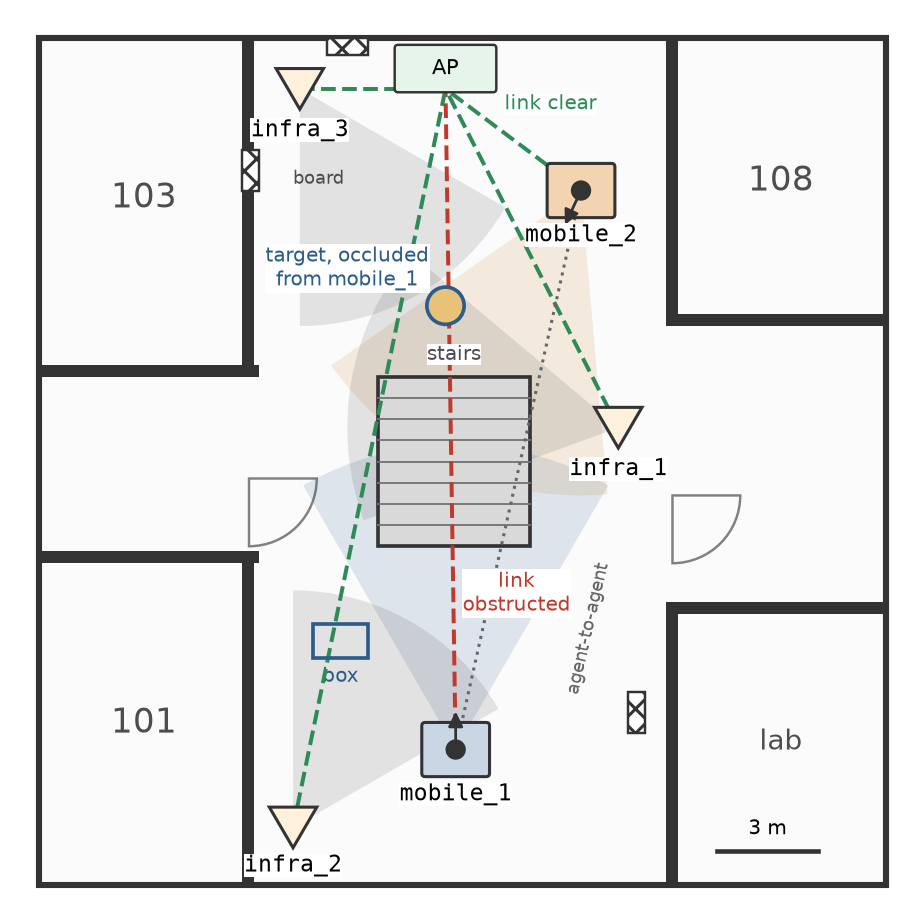
\includegraphics[width=\columnwidth]{figs/fig01_overview.png}
\caption{A recording scenario, top view.}
\label{fig:overview}
\end{figure}

\subsection{Design Principles}
Four decisions shape the system and recur throughout the paper.

\emph{The link is a measurement, not a transport.} Each unit records
locally; no sensor stream traverses the wireless network before
reaching disk. The only traffic the testbed itself places on the link
is clock synchronization and the active probes of
Sec.~\ref{sec:comm}, both of which are present in every run and
therefore form part of the channel that is measured. This keeps the
measured link representative of what a deployed team would have, and
keeps a link outage from costing sensor data.

\emph{Rigs are fixed; calibration is done once.} In each agent, a fixed
rig compounds the multi-modal sensors (Fig.~\ref{fig:platforms}). The
rig is constant across all recordings, removing the need to calibrate
in every session, and allowing each extrinsic to be validated on
observations that did not enter its estimation
(Sec.~\ref{sec:calibration}).

\emph{One frozen map per site places every agent.} A dense reference
map built with the testbed's own LiDAR is frozen before any sequence
is recorded. LiDAR agents enter the map frame by scan-to-map
registration; agents without a LiDAR enter it through fiducial boards
whose poses were themselves estimated from the map
(Sec.~\ref{sec:groundtruth}). No survey instrument is required.

\emph{Every reference quantity is validated out of sample.} Extrinsics,
clock offsets, and poses are each checked against data that did not
inform them: held-out boards and reflector positions, probe packets
stamped on both ends, a second mapping pass, and laser-rangefinder
control distances.

\subsection{Agents}
\texttt{mobile\_1} is an AgileX Scout Mini equipped with an Ouster
LiDAR, a ZED~2i stereo camera with an integrated IMU, two IWR6843
mmWave radars, and an RTL8852BU Wi-Fi interface. It also carries
\texttt{sniffer}, a Raspberry Pi~4 whose BCM43455c0 chipset is used
for CSI extraction. \texttt{mobile\_2}, the sensor-constrained agent,
is a pushcart equipped with a RealSense D455 RGB-D camera with IMU, an
on-board visual SLAM pipeline, and a Wi-Fi interface \todo{Add Radar
(?)}. Each infrastructure agent, \texttt{infra\_N}, is a mast with an
Arducam RGB camera, an IWR6843 radar, and a Raspberry Pi whose
on-board BCM43455 serves as the wireless interface. The sensor models,
rates, and resolutions are listed in Table~\ref{tab:sensors}.

\begin{figure*}[t]
\centering
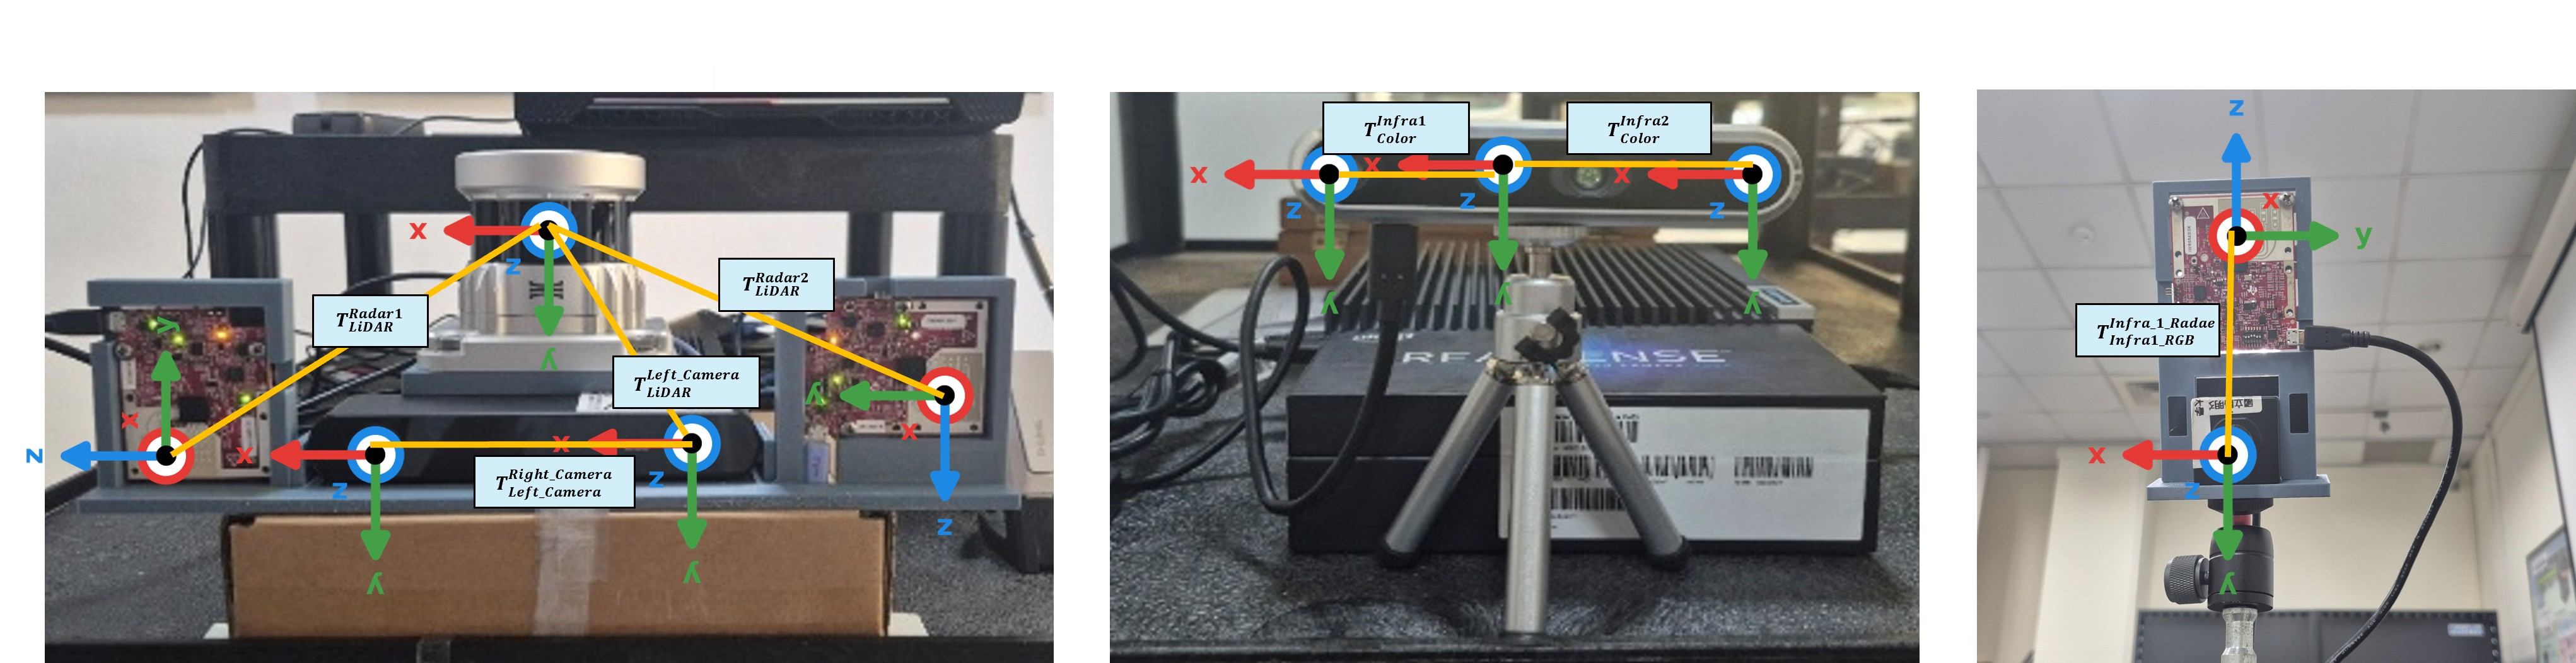
\includegraphics[width=\textwidth]{figs/fig02_platforms.jpg}
\caption{Platforms and frames. Axes mark each sensor frame (x red,
y green, z blue); yellow arrows are the extrinsic transforms
estimated in Sec.~\ref{sec:alignment}. \texttt{mobile\_1} uses
\texttt{base\_link} as origin (not shown here), \texttt{mobile\_2} its LiDAR, and the
infrastructure rig its camera.}
\label{fig:platforms}
\end{figure*}

\begin{table*}[!t]
\caption{Per-Agent Sensor Specifications}
\begin{center}
\renewcommand{\arraystretch}{1.2}
\setlength{\tabcolsep}{4pt}
\scriptsize
\begin{tabular}{@{}p{2.0cm} p{2.6cm} p{5.6cm} p{1.9cm} p{2.1cm} p{1.5cm}@{}}
\toprule
\textbf{Equipment} & \textbf{Model Type} & \textbf{Characteristics} & \textbf{Resolution} & \textbf{FoV} & \textbf{Rate} \\
\midrule
\multicolumn{6}{@{}l}{\textit{Mobile Agents}} \\
LiDAR & Ouster OS1-128 & 100 m range & 1024 $\times$ 128 & 45$^\circ$ vert. & 10 Hz \\
LiDAR & Ouster OS0-64 & 50 m range & 1024 $\times$ 64 & 90$^\circ$ vert. & 10 Hz \\
Stereo Camera & ZED 2i & RGB stereo, baseline 120 mm & 1920 $\times$ 1080 & 110$^\circ$ $\times$ 70$^\circ$ & 30 Hz \\
 & & IMU 6-axis, barometer, magnetometer & -- & -- & 400 Hz \\
RGBD & RealSense D455 & RGB, global shutter & 1280 $\times$ 800 & 90$^\circ$ $\times$ 65$^\circ$ & 30 Hz \\
 & & Stereo IR, global shutter, baseline 95 mm & 1280 $\times$ 720 & 87$^\circ$ $\times$ 58$^\circ$ & 30 Hz \\
 & & IMU BMI 055 & -- & -- & 200 Hz \\
 Radar & TI IWR6843ISK & 60--62 GHz, 3 TX / 4 RX & \shortstack[l]{7.5\,cm range \\ $14.2^\circ$ az., $57^\circ$ el.} & $\pm$60$^\circ$ az., $\pm$20$^\circ$ el & 10 Hz \\
Radar & TI IWR6843ISK & 62--64 GHz, 3 TX / 4 RX & \shortstack[l]{7.5\,cm range \\ $13.8^\circ$ az., $55^\circ$ el.} & $\pm$60$^\circ$ az., $\pm$20$^\circ$ el & 10 Hz \\
Radar & TI MMWCAS-RF-EVM & 76--81 GHz, 4$\times$ AWR2243 cascade, 12 TX / 16 RX & \todo{--} & \todo{--} & \todo{--} Hz \\
CSI extractor & RPi 4B (BCM43455c0) & Nexmon, monitor mode, 80 MHz, 1 antenna & 256 subcarriers & -- & $\sim$100 Hz \\
Wi-Fi USB Dongle &  D-Link AX1800 & USB, 5 GHz 802.11ac; iw / iperf3 endpoint & -- & -- & 5/1 Hz \\
Computer &  MIC-713-OX4B2 & NVIDIA Jetson AGX Orin & -- & -- & -- \\

\midrule
\multicolumn{6}{@{}l}{\textit{Infrastructure Agents}} \\
RGB Camera & Arducam B0495 & AR0234, color global shutter, M12 lens & 1920 $\times$ 1200 & 95$^\circ$ diag. & 30 Hz \\
Radar & TI IWR6843ISK & 61.75--64 GHz, 3 TX / 4 RX & \shortstack[l]{7.5\,cm range \\ $13.9^\circ$ az., $56^\circ$ el.} & $\pm$60$^\circ$ az., , $\pm$20$^\circ$ & 10 Hz \\
CSI extractor & RPi 4B (BCM43455c0) & Nexmon, monitor mode, 80 MHz, 1 antenna & 256 subcarriers & -- & $\sim$100 Hz \\
Wi-Fi USB Dongle & Edimax N150 & USB, 5 GHz 802.11ac; iw / iperf3 endpoint & -- & -- &  5/1 Hz \\

\bottomrule
\end{tabular}
\end{center}
\label{tab:sensors}
\end{table*}


The heterogeneity is deliberate. \texttt{mobile\_1} is the fully
equipped agent whose LiDAR builds the reference map.
\texttt{mobile\_2} represents the class of low-cost agents that a
deployed team will contain and that a reference pipeline must be able
to localize without a LiDAR. The infrastructure agents provide the
elevated, persistent vantage that no mobile node can sustain, and the
camera-only sensing typical of fixed installations.

\subsection{Frames}
\label{sec:frames}
The sensors of each platform are expressed in the origin frame of that
platform, and each platform is expressed in the world frame of its
site (Sec.~\ref{sec:groundtruth}). The origin frame depends on the
platform. For \texttt{mobile\_1} we use the robot's
\texttt{base\_link}, so that sensor data and poses are expressed
relative to the body that moves and can be related to wheel odometry
and control. \texttt{mobile\_2} has no robot body, so its LiDAR is
used as the origin, as it provides the strongest metric. For the
infrastructure agents, which carry no LiDAR, the origin is the camera.
The estimation of each transform is described in
Sec.~\ref{sec:calibration}.

\subsection{Recording}
\label{sec:recording}
Each unit records what its sensors and interfaces produce, and nothing
else: Ouster packets with the sensor's metadata message, images and
IMU samples, radar detections, the on-board visual SLAM output of
\texttt{mobile\_2}, the wireless metrics of Sec.~\ref{sec:comm}, and
the raw Nexmon CSI frames on \texttt{sniffer}. Decoded clouds,
reference poses, and parsed CSI do not exist at recording time; they
are produced by the post-processing of Sec.~\ref{sec:postproc}.
Table~\ref{tab:topics} lists the recorded topics per unit.

Ouster data is stored as raw packets together with the sensor's
metadata message, which allows lossless re-decoding through the vendor
driver at any later time. \texttt{mobile\_2} provides an RGB-D module
(color, aligned depth, and both infrared imagers with
\texttt{CameraInfo} and factory extrinsics) and the full output of its
on-board GPU visual SLAM pipeline, including the drifting
visual-odometry path, the loop-closed path, and the tracker status.
Infrastructure units provide an RGB camera and a radar each. The
wireless measurements appear as ordinary topics on the same timeline,
and the CSI stream from \texttt{sniffer} is recorded in its own bag as
raw Nexmon frames.

\begin{table*}[!t]
\caption{Recorded topics per unit (representative rates).}
\label{tab:topics}
\begin{center}
\renewcommand{\arraystretch}{1.2}
\setlength{\tabcolsep}{4pt}
\scriptsize
\begin{tabular}{@{}p{6.2cm} p{6.6cm} p{2.6cm}@{}}
\toprule
\textbf{Topic (namespace)} & \textbf{Message Type} & \textbf{Rate} \\
\midrule
\multicolumn{3}{@{}l}{\textit{\texttt{mobile\_1/}}} \\
\texttt{ouster/lidar\_packets} & \texttt{ouster\_sensor\_msgs/PacketMsg} & 640 Hz \\
\texttt{ouster/imu\_packets} & \texttt{ouster\_sensor\_msgs/PacketMsg} & 100 Hz \\
\texttt{ouster/metadata} & \texttt{std\_msgs/String} & latched \\
\texttt{radar\{1,2\}/radar/points\_all} & \texttt{PointCloud2} & 10 Hz \\
\texttt{zed/left/image\_rect\_color} & \texttt{Image} (+\,\texttt{CameraInfo}) & 15 Hz \\
\texttt{zed/depth/depth\_registered} & \texttt{Image} & 15 Hz \\
\texttt{zed/imu/data}, \texttt{zed/imu/mag} & \texttt{Imu}, \texttt{MagneticField} & 200 / 50 Hz \\
\texttt{zed/odom}, \texttt{zed/pose}, \texttt{zed/path\_*} & \texttt{Odometry}, \texttt{PoseStamped}, \texttt{Path} & 15 Hz \\
\texttt{tf}, \texttt{tf\_static} & \texttt{TFMessage} & --- \\
\addlinespace
\multicolumn{3}{@{}l}{\textit{\texttt{mobile\_2/}}} \\
\texttt{color/image\_raw} & \texttt{Image} (+\,\texttt{CameraInfo}) & 30 Hz \\
\texttt{depth/image\_rect\_raw} & \texttt{Image} (+\,\texttt{CameraInfo}) & 30 Hz \\
\texttt{infra\{1,2\}/image\_rect\_raw} & \texttt{Image} (+\,\texttt{CameraInfo}) & 30 Hz \\
\texttt{extrinsics/depth\_to\_infra\{1,2\}} & \texttt{realsense2\_camera\_msgs/Extrinsics} & latched \\
\texttt{imu} & \texttt{Imu} & 200 Hz \\
\texttt{visual\_slam/tracking/*}, \texttt{status} & \texttt{Odometry}, \texttt{PoseStamped}, \texttt{Path} & 30 Hz \\
\addlinespace
\multicolumn{3}{@{}l}{\textit{\texttt{infra\_N/}}} \\
\texttt{image\_raw} & \texttt{Image} (+\,\texttt{CameraInfo}) & 30 Hz \\
\texttt{radar/points\_all} & \texttt{PointCloud2} & 10 Hz \\
\addlinespace
\multicolumn{3}{@{}l}{\textit{\texttt{sniffer/}}} \\
\texttt{csi} & \unsure{\texttt{csi\_msgs/Csi}} & $\sim$100--140 Hz \\
\addlinespace
\multicolumn{3}{@{}l}{\textit{All units}} \\
\texttt{wifi/status} & \texttt{wifi\_monitor\_msgs/WifiLinkStatus} & 5 Hz \\
\texttt{wifi/iperf}, \texttt{wifi/iperf\_r2r} & \texttt{wifi\_monitor\_msgs/IperfResult} & per test \\
\texttt{ntp/status}, \texttt{ntp/events} & \texttt{ntp\_monitor\_msgs/NtpStatus}, \texttt{String} & 10 Hz / event \\
\bottomrule
\end{tabular}
\end{center}
\end{table*}


%=======================================================================
\section{Calibration and Timing}
\label{sec:calibration}
Two calibrations are required to relate the streams. The spatial
calibration places every sensor in the origin frame of its platform.
The temporal calibration places every measurement on a common
timeline. Each is validated with data that was not used in its
estimation. The placement of platforms in the world frame is part of
the reference and is described in Sec.~\ref{sec:groundtruth}.

\subsection{Spatial Calibration}
\label{sec:spatial}
Three transforms are estimated per platform. On \texttt{mobile\_1},
\Ttransform{Base}{LiDAR} is obtained by hand-eye calibration: the
robot is driven through a sequence of motions, and the transform is
solved from the pairs of relative motions reported by wheel odometry
and by LiDAR odometry \cite{furrer2018handeye}. On both mobile
agents, \Ttransform{LiDAR}{Camera} is obtained by direct, target-free
alignment of image and point-cloud features \cite{koide2023lidarcam}.
For the radar, whose returns are too sparse for feature alignment,
\Ttransform{LiDAR}{Radar} is obtained with a corner reflector placed
at several positions \cite{domhof2019calib}.

For the infrastructure rig, the camera and radar are mounted on the
same fixed bracket and each sensor is calibrated against a LiDAR by
the same methods, which gives \Ttransform{Camera}{Radar} directly.
Since the rig is fixed, the extrinsic remains valid once the sensors
are placed on the infrastructure. The world pose of each
infrastructure camera is obtained during the mapping session through
the fiducial chain of Sec.~\ref{sec:fiducials}.

\subsection{Temporal Calibration}
\label{sec:temporal}
Each unit records its own bag, so frames from different agents are
related only through their timestamps. Two conditions must hold: the
clocks of the units must agree, and each stamp must be close to the
time at which its measurement was taken. We address each condition
below and then bound the remaining error.

\subsubsection{Clock Synchronization}
The clocks are synchronized with chrony. \texttt{mobile\_1} acts as
the server, and every other agent and \texttt{sniffer} act as clients
polling every \SI{8}{\second}. This traffic passes over the measured
link, but at a few hundred bytes per poll it is negligible, and since
it is present in every run it forms part of the measured channel.
Recording starts only after every unit reports a converged offset.
Each unit logs its offset and any clock adjustment
(\texttt{ntp/status}, \texttt{ntp/events}) into its own bag, so the
alignment at any frame can be checked and poorly aligned frames can
be filtered out.

Table~\ref{tab:ntp} summarizes the result over \todo{1} sequences. No
clock was stepped during any recording, and the worst pairwise offset
is \todo{about \SI{70}{\micro\second}}.

\begin{table}[t]
\centering
\caption{Clock synchronization across all sequences (server:
\texttt{mobile\_1}). 
\todo{Values from a single live pass; update once all sequences are processed.}}
\label{tab:ntp}
\footnotesize
\begin{tabular}{@{}lccccc@{}}
\toprule
& \multicolumn{2}{c}{RMS offset} & & & \\
\cmidrule(lr){2-3}
Client & Median & Max & Jitter (med.) & Path delay (med.) & Steps \\
\midrule
\texttt{mobile\_2} & \SI{10.9}{\micro\second} & \SI{10.9}{\micro\second} & \SI{227}{\micro\second} & \SI{4.2}{\milli\second}  & 0 \\
\texttt{infra\_1}  & \SI{42.5}{\micro\second} & \SI{42.5}{\micro\second} & \SI{175}{\micro\second} & \SI{4.1}{\milli\second}  & 0 \\
\texttt{sniffer}   & \SI{28.7}{\micro\second} & \SI{28.7}{\micro\second} & \SI{619}{\micro\second} & \SI{15.6}{\milli\second} & 0 \\
\bottomrule
\end{tabular}
\end{table}


These offsets describe the stability of each clock relative to the
server, not its accuracy. NTP assumes a symmetric path delay, and any
asymmetry appears as a constant bias that chrony cannot observe. This
is relevant only for \texttt{sniffer}, which reaches the server over
its \SI{2.4}{\giga\hertz} management link with a path delay several
times larger than that of the other units, so its bias may be as
large as half that delay, \SI{7.8}{\milli\second}. We measure the
bias directly from the probe packets that \texttt{mobile\_2} sends
and \texttt{sniffer} captures. Each packet is stamped at transmission
on the clock of \texttt{mobile\_2} and at reception on the clock of
\texttt{sniffer}. Since the packet is in flight for only nanoseconds,
the difference between the two stamps equals the bias of the sniffer
plus its driver latency. The median difference over a run is
\todo{}, which bounds the bias. \todo{Remove this consideration by
replacing the connection to the sniffer with Ethernet directly to
mobile\_1; see Sec.~\ref{sec:lessons}.}

\subsubsection{Timestamp Latency}
Agreeing clocks are not sufficient if the stamps themselves are
late. Every message is stamped on arrival at its host, so each stamp
lags its measurement by the transport latency of that sensor
\todo{estimates per sensor: LiDAR over Ethernet, cameras over USB,
radar over UART}, and camera stamps lag further by the exposure time.
These lags are approximately constant for a given sensor. We leave
the stamps as recorded so that users can apply their own correction,
for example by aligning the motion observed by each sensor.

\subsubsection{Motion Compensation and Fusion Error Bounds}
\label{sec:temporal_bounds}
Both conditions reduce to a timing error $\Delta t$, which displaces
a measurement taken on a platform moving at speed $v$ by
\begin{equation}
  \delta x = v \, \Delta t .
  \label{eq:time_bound}
\end{equation}
We take $v_{\max} = \SI{3}{\metre\per\second}$ as an upper bound on
agent speed. The clock offset of \unsure{\SI{70}{\micro\second}} then
corresponds to \unsure{\SI{0.21}{\milli\metre}}, and the sniffer bias
of \todo{} to \todo{}, which is \todo{}\,\% of the half-wavelength
$\lambda/2 = \SI{26.1}{\milli\metre}$ at \SI{5745}{\mega\hertz} that
sets the CSI sampling requirement (Sec.~\ref{sec:csi}). Transport
latency and exposure are larger: a constant lag of
\SI{10}{\milli\second} corresponds to \SI{3}{\centi\metre}, but since
it is constant it can be estimated and removed. The largest term is
the LiDAR sweep, which takes \SI{100}{\milli\second} at
\SI{10}{\hertz}, so the first and last points of a scan can be
\SI{30}{\centi\metre} apart. This is removed by per-point deskewing
with IMU-propagated motion in the reference pipeline \cite{glim}.

Combining the terms that remain after compensation, the worst-case
intra-frame spatial error at $v_{\max}$ is
\begin{equation}
  \delta x_{\max} = v_{\max}\,\big(\Delta t_{\mathrm{clk}}
  + \Delta t_{\mathrm{lat}} + \Delta t_{\mathrm{exp}}\big)
  = \todo{Y}\,\si{\centi\metre},
  \label{eq:fusion_bound}
\end{equation}
where $\Delta t_{\mathrm{clk}}$ is the worst clock offset,
$\Delta t_{\mathrm{lat}}$ the largest uncorrected transport latency,
and $\Delta t_{\mathrm{exp}}$ the longest camera exposure. The LiDAR
sweep is excluded because it is deskewed.

The error budget is therefore dominated by sensor physics and
transport, not by synchronization. Clock alignment contributes well
under a millimetre, while the larger terms are either compensated,
as for the LiDAR sweep, or constant and removable, as for per-sensor
latency.

\subsection{Calibration Validation}
\label{sec:calib_val}
Each extrinsic is checked on data that was not used in its
estimation. For \Ttransform{LiDAR}{Camera}, the LiDAR returns on the
ChArUco boards of the mapping session are projected into the image
and compared with the detected board corners; the reprojection
residual is reported per board and per range. For the RGB-D agent,
whose trajectory uses board sightings as constraints, the boards are
split once per site into an estimation set and a held-out set, and
the residual is evaluated on the held-out set only. \todo{State the
split, e.g. every third board.}

For \Ttransform{LiDAR}{Radar}, the corner reflector is placed at
positions not used in calibration, and the radar detection is
compared with the LiDAR centroid of the reflector. For
\Ttransform{Base}{LiDAR}, the hand-eye result is checked through the
board residual of Sec.~\ref{sec:gt_val}: a board observed from
\texttt{mobile\_1} predicts a board pose through
\Ttransform{Base}{LiDAR} and \Ttransform{LiDAR}{Camera}, so the
residual tests both transforms at once and is not reported
separately. For the infrastructure rig, \Ttransform{Camera}{Radar} is
checked in the same way as the mobile radar, with the rig mounted in
place. Table~\ref{tab:calib} lists the residuals per sensor pair. The
same values are stored with the released data
(\texttt{calibration/residuals.json}) so that users can weight each
transform according to its accuracy.

\begin{table}[t]
\centering
\caption{Calibration residuals on held-out observations.}
\label{tab:calib}
\footnotesize
\setlength{\tabcolsep}{4pt}
\begin{tabular}{@{}llll@{}}
\toprule
Transform & Check & Median & p95 \\
\midrule
\Ttransform{LiDAR}{Camera}  & board corner reprojection (px) & \todo{} & \todo{} \\
\Ttransform{LiDAR}{Radar}   & reflector offset (cm)          & \todo{} & \todo{} \\
\Ttransform{Base}{LiDAR}    & board pose via chain (cm, deg) & \todo{} & \todo{} \\
\Ttransform{Camera}{Radar}  & reflector offset (cm), infra   & \todo{} & \todo{} \\
Clock, all clients          & offset to \texttt{mobile\_1} (\si{\micro\second}) & \todo{} & \todo{} \\
Clock, \texttt{sniffer}     & probe-packet bias (ms)         & \todo{} & \todo{} \\
\bottomrule
\end{tabular}
\end{table}


%=======================================================================
\section{Reference Localization}
\label{sec:groundtruth}
The reference combines three of the strategies reviewed in
Sec.~\ref{sec:gt_related}. The reference map is SLAM-derived, which
removes the survey scanner normally required for map registration.
Every scan is registered against this map, so the pose is carried by
the map and not by odometry between anchors. Fiducial boards, posed
in the map frame during the mapping session, anchor the RGB-D agent
and the infrastructure where registration alone is weak. Since the
annotations of the dataset \cite{scoop_dataset} are derived from these
poses, the reference is built and validated to annotation grade and
not only as an evaluation target. Fig.~\ref{fig:refpipeline} shows the
pipeline; the following subsections describe each stage.

\begin{figure*}[t]
\centering
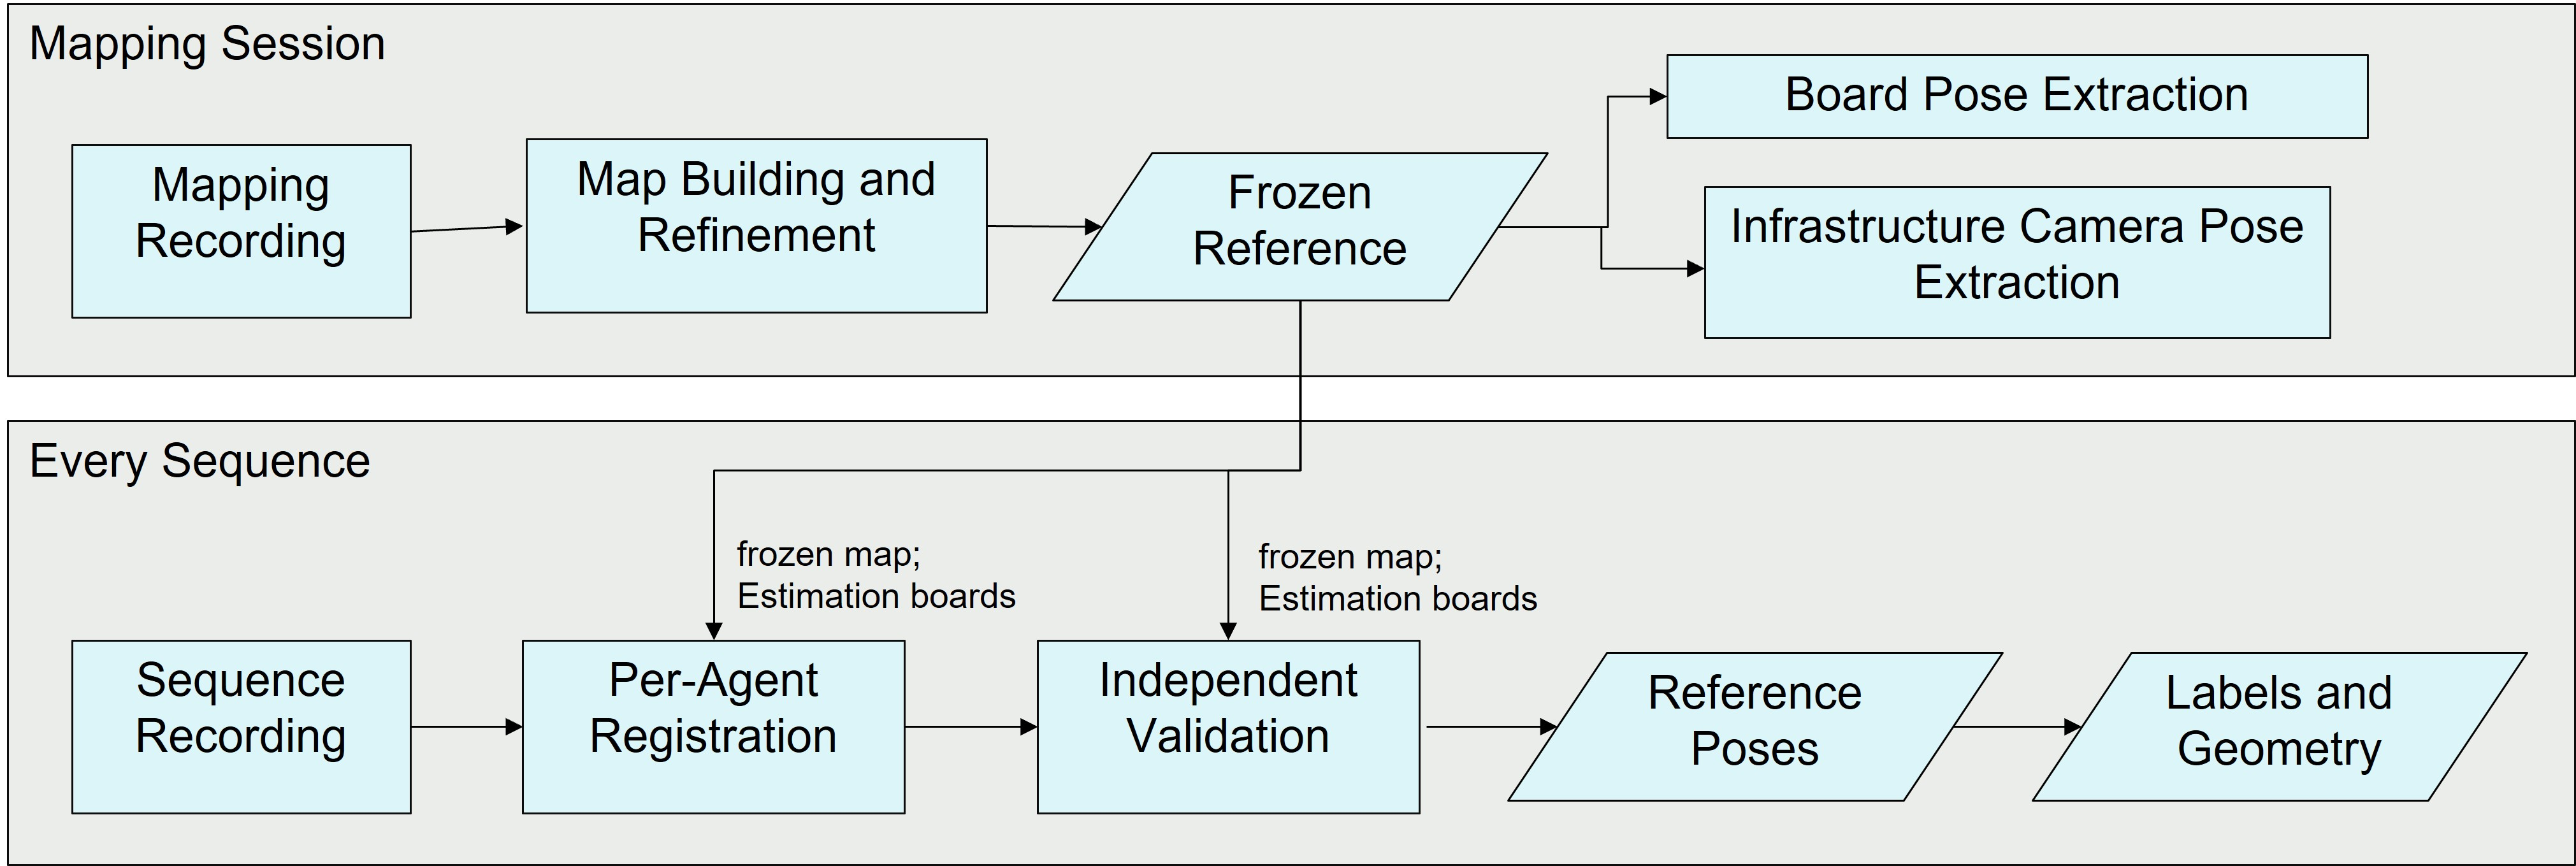
\includegraphics[width=\textwidth]{figs/fig_refpipeline.jpg}
\caption{Reference pipeline. Top: the mapping session, run once per
site, builds and refines the map, poses the boards in it
(Eq.~\eqref{eq:board_chain}), and places the infrastructure cameras
through the boards (Eq.~\eqref{eq:infra_camera_chain}). Bottom: each
sequence is registered into the frozen map, by scan-to-map ICP for the
LiDAR agents and by odometry with ICP and board factors for the RGB-D
agent, and the poses are exported in the site frame.}
\label{fig:refpipeline}
\end{figure*}

\subsection{Reference Map and Scan-to-Map Registration}
\label{sec:gt}
The reference map is built in a dedicated mapping session and held
fixed afterwards; no recorded sequence contributes to it. A second,
separate mapping pass is recorded and processed independently and is
used only to cross-check the first. A LiDAR-inertial SLAM solution
\cite{glim} estimates the mapping trajectory, with sub-mapping and
loop closure tuned for offline accuracy and checked so that no submap
is left without a long-range constraint. The map is then frozen and
every scan is re-registered into it by point-to-plane ICP against
local plane fits, iterated until the pose corrections fall below the
sensor noise. This follows the prior-map registration used by the
survey-grade datasets \cite{newercollege,oxfordspires,lamar}, with
the prior built by our own sensors instead of a survey scanner. Plane
fits are used instead of nearest-neighbour targets because, on a
surface smeared by accumulated drift, a \SI{3.0}{\centi\metre} scan
offset produces only \SI{0.5}{\centi\metre} of nearest-neighbour
residual, so the error would not be visible to conventional ICP.

This frozen map is the metric backbone of every sequence. The
LiDAR-equipped agents are localized by scan-to-map registration. For
\texttt{mobile\_2}, the depth registration, its visual odometry, and a
subset of the board sightings of Sec.~\ref{sec:fiducials} are
combined in one pose-graph optimization per sequence, with the
selected boards entering as absolute pose factors; the remaining
boards are held out and serve only for validation
(Sec.~\ref{sec:gt_val}). The LiDAR agents need no board factors,
since scan-to-map registration alone constrains every frame, so for
them every board sighting is a validation measurement. \unsure{All
trajectories therefore share one metric frame by construction and do
not require post-hoc alignment.} Inter-agent relative poses reduce to
two registration errors against shared local geometry instead of two
accumulated drifts, and since no recorded sequence contributes to the
map, the agreement of each agent with the map is an out-of-sample
check.

\begin{figure}[t]
\centering
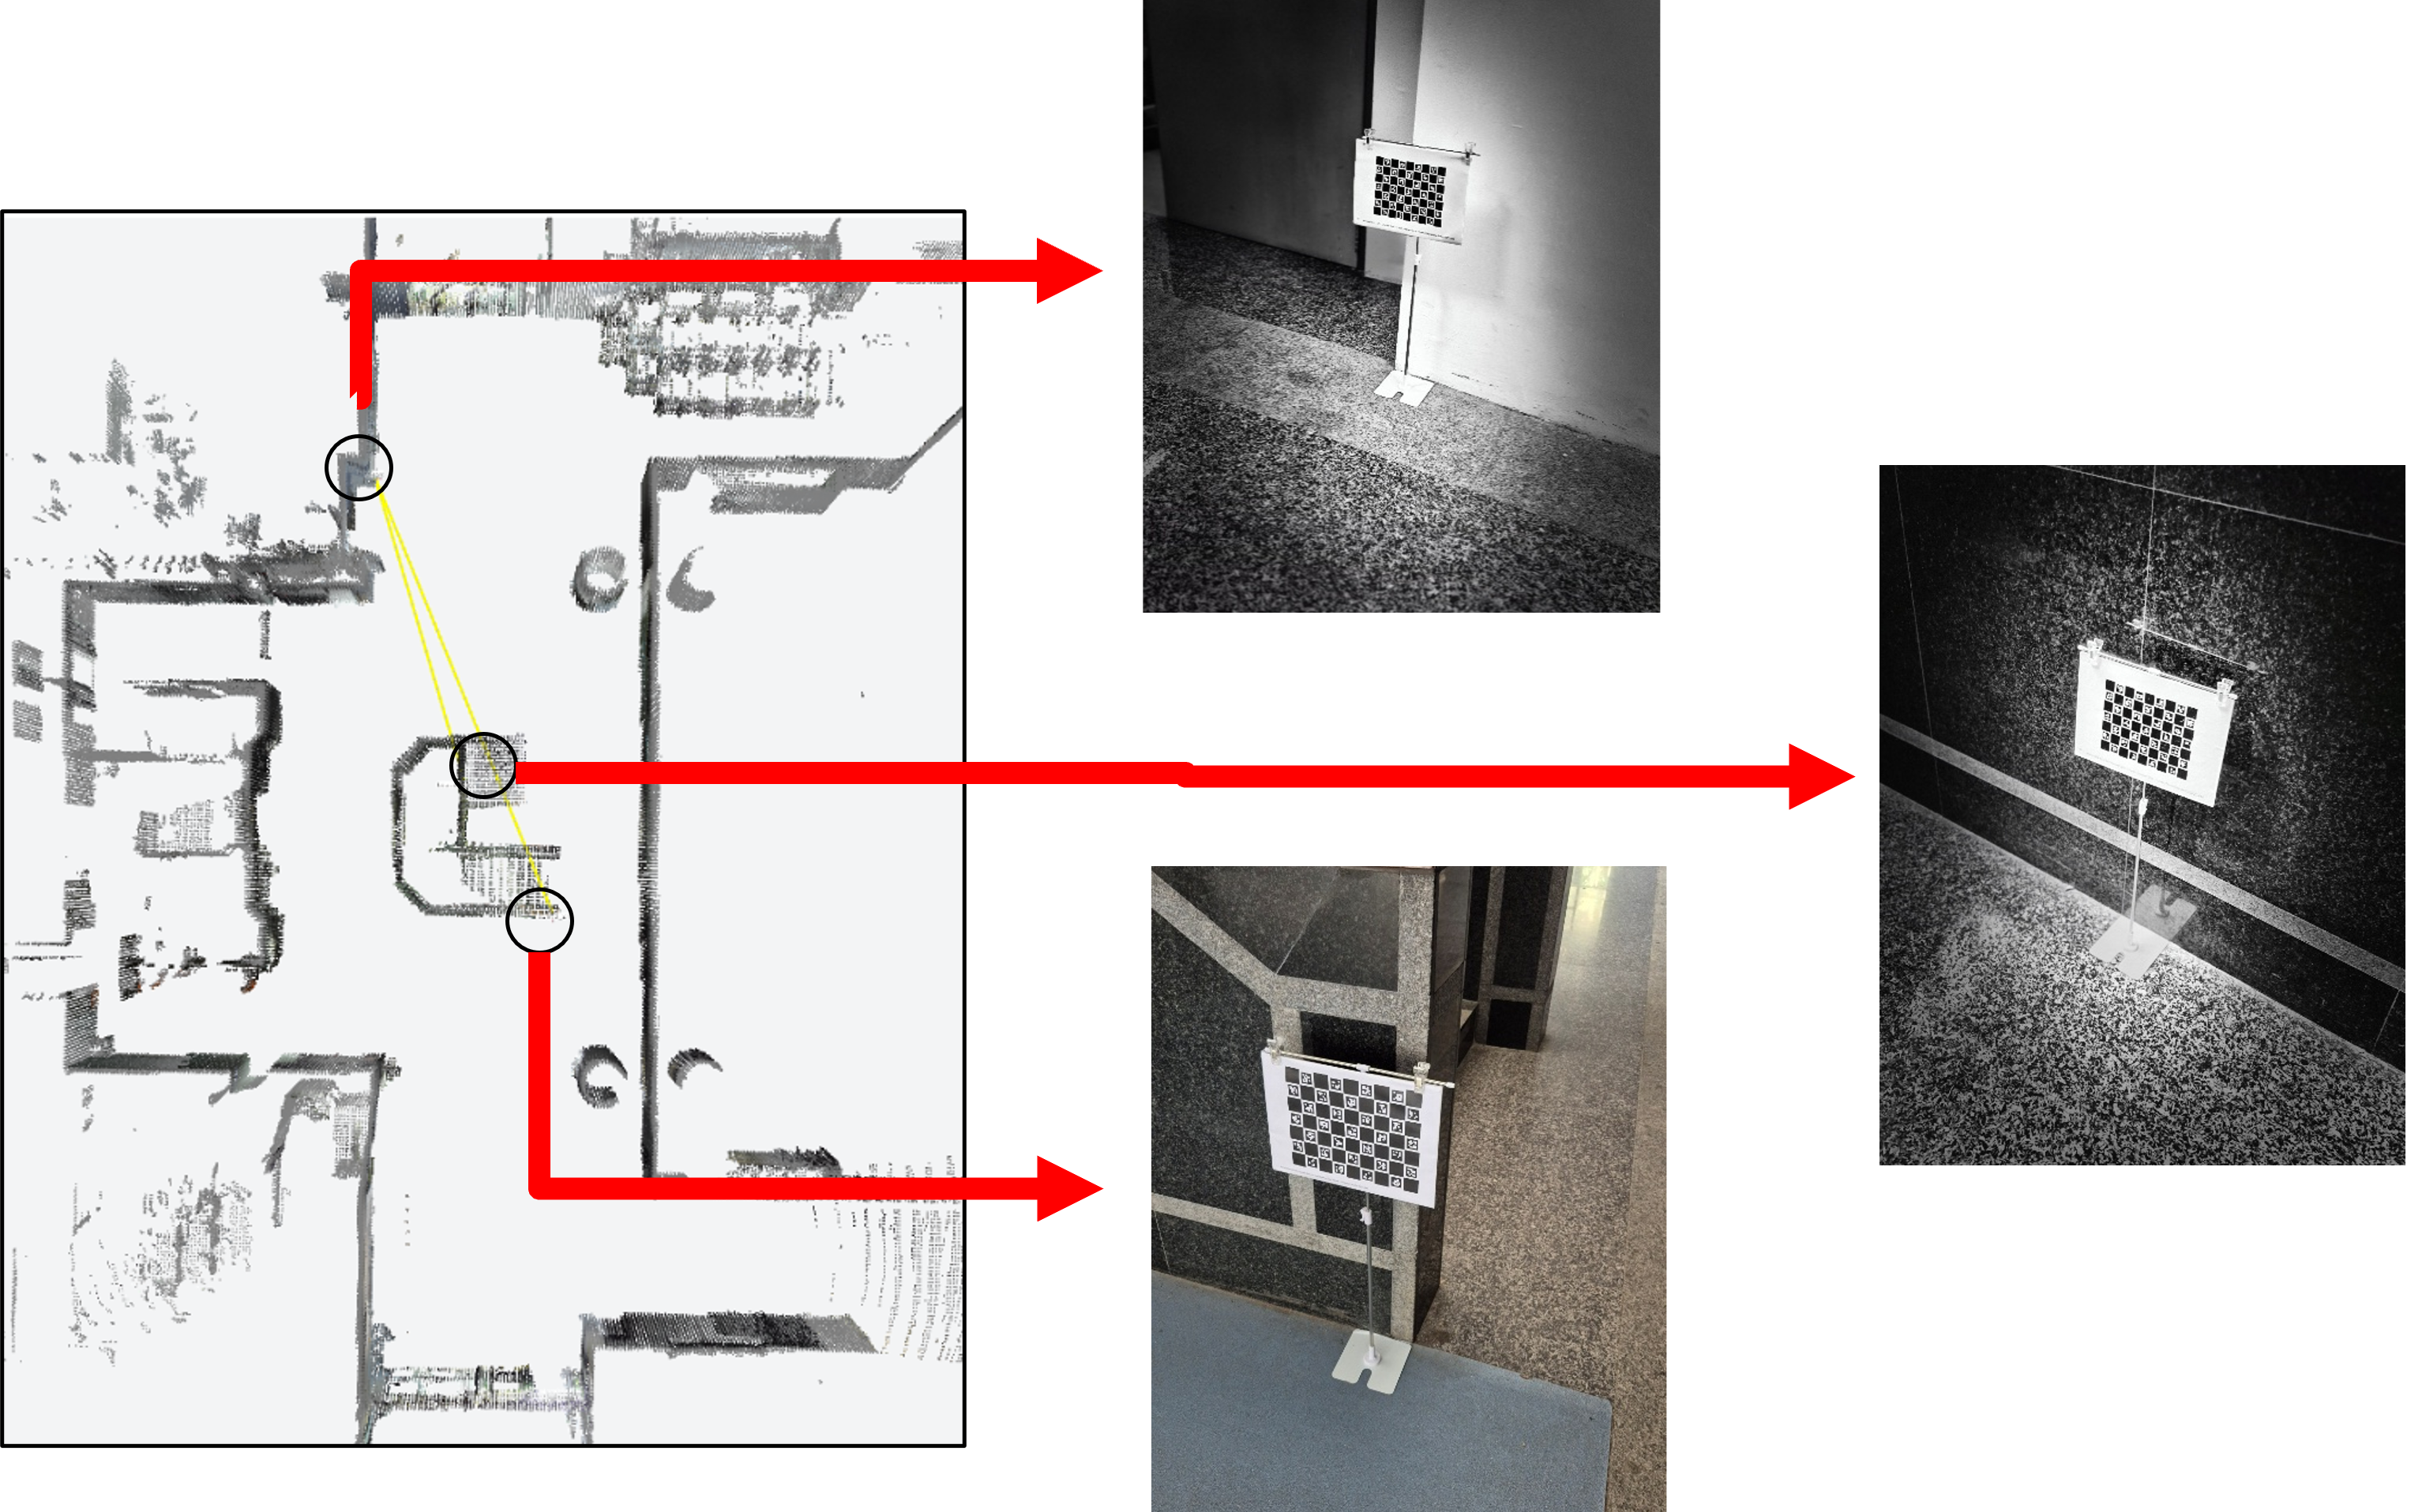
\includegraphics[width=\columnwidth]{figs/fig_refpipeline_output.png}
\caption{Reference map with the fiducial network}
\label{fig:refmap}
\end{figure}


\subsection{Fiducial Network}
\label{sec:fiducials}
The reference map provides the shared metric frame, but a
sensor-constrained agent cannot enter it by registration alone. A
cold-start ICP against a building-scale map may converge in a wrong
basin, and between registrations the visual odometry of the agent
accumulates drift, fastest in feature-poor regions where the local
geometry only weakly constrains the alignment. We therefore deploy a
network of printed ChArUco boards in the environment. The boards are
not surveyed independently: the pose of each board is estimated in
the reference frame from the observations of the mapping session
itself, so the network inherits the metric accuracy of the map. This
is sparse anchoring as in \cite{airmuseum}, with the anchors posed by
the map instead of by survey equipment.

During the mapping session, the mapping agent, which carries a LiDAR
and a camera, loops around the site and stops at each board to
record several views of it. With the mapping trajectory
\Ttransform{World}{LiDAR} from Sec.~\ref{sec:gt} and the extrinsic
\Ttransform{LiDAR}{MobileCamera} from Sec.~\ref{sec:spatial}, the
pose of each board is
\begin{equation}
   \Ttransform{World}{Board} = \Ttransform{World}{LiDAR} \times \Ttransform{LiDAR}{MobileCamera} \times \Ttransform{MobileCamera}{Board} .
   \label{eq:board_chain}
\end{equation}
One board serves as the origin of the world frame,
\Ttransform{World}{OriginBoard}, and every mobile agent starts at a
board, so that each run begins at a known pose.

Infrastructure agents are placed in the same frame through the
boards. During the mapping session, a
\(500\,\mathrm{cm} \times 500\,\mathrm{cm}\) ChArUco board is shown to
the mobile and infrastructure cameras simultaneously in the same
frame. Each camera computes its pose relative to the board,
\Ttransform{Board}{MobileCamera} and \Ttransform{Board}{InfraCamera},
and the world pose of the infrastructure camera is
\begin{equation}
\begin{split}
  \Ttransform{World}{InfraCamera} = {}
    & \Ttransform{World}{LiDAR} \times \Ttransform{LiDAR}{MobileCamera} \times \\
    &  (\Ttransform{Board}{MobileCamera})^{-1} \times \Ttransform{Board}{InfraCamera} .
\end{split}
\label{eq:infra_camera_chain}
\end{equation}

The boards serve three roles. At the start of a sequence, a board
sighting provides the absolute initial pose that places the first
registration in the correct convergence basin. Along the trajectory,
board sightings provide absolute pose observations that bound the
drift accumulated by visual odometry between map registrations.
\unsure{For this reason the boards are placed mainly in feature-poor
regions, where both visual tracking and depth registration are
weakest.} Finally, the boards are used to validate the registration
of every subsequent sequence, as described in Sec.~\ref{sec:gt_val}.

\subsection{Validation Methodology}
\label{sec:gt_val}
Convergence of the refinement in Sec.~\ref{sec:gt} establishes
self-consistency, not accuracy. The plane targets are themselves
estimated from the map, so a self-consistent deformation would
converge equally well. Accuracy is therefore established by checks
that did not enter the estimation, along two axes: where the surfaces
are, and how consistently the poses place them. The results are
reported in Sec.~\ref{sec:eval_gt}.

\paragraph{Second mapping pass.} Surfaces are measured by their
thickness, defined as the p95--p5 spread of points about planes
fitted to \SI{0.25}{\metre} patches, and always compared with the
sensor noise floor obtained from individual sweeps, which carry no
pose error. A second recording, captured weeks later and processed
independently, is compared in surface placement and relative scale.
Since both runs share the sensor and the algorithm, this establishes
scale \emph{stability} between sessions; a deformation common to both
would not be visible in this test.

\paragraph{Control distances.} The absolute scale is established by
laser-rangefinder control distances measured between landmarks such
as walls at each site. Their disagreement with the map grows with the
scale at which a common deformation would act, which closes the gap
left by the second pass.

\paragraph{Held-out boards.} The pose of each board in the map is
fixed by the mapping session. When an agent sights a board during a
sequence, its registered pose and camera extrinsic predict where the
board should appear, and the difference between this prediction and
the observed board pose is a residual that did not enter the
registration. It is therefore an independent check at that frame.
For the RGB-D agent, whose trajectory uses board sightings as
constraints, a subset of boards is held out of the estimation and the
residual is evaluated on those boards only.

\paragraph{Pose consistency.} Per-scan consistency is measured where
the same surface is observed twice: by the same robot minutes apart,
and by different robots on overlapping routes. The second case tests
the full chain of each robot (registration, extrinsic calibration,
and time association) at LiDAR accuracy for the LiDAR pair, and
isolates the sensor-constrained mechanism for the RGB-D robot.

%=======================================================================
\section{Communication Measurement}
\label{sec:comm}
The link is recorded on the same timeline as the sensing streams at
two levels: the link state, which describes what the network
delivered, and the channel state, which describes the propagation
that produced it. Fig.~\ref{fig:linktrace} shows one sequence.

\subsection{Network Configuration}
All agents associate to a single access point on channel 149 (VHT-80,
\SI{5745}{\mega\hertz}); no ad hoc or mesh mode is used. The
transmitter settings are imposed by the CSI receiver: 1$\times$1
802.11ac configuration. 802.11ax is disabled, since the receiver
cannot demodulate HE frames and would capture only control frames,
and the number of spatial streams is fixed to one, since a
single-antenna receiver cannot separate a two-stream transmission.
Power save is disabled on all transmitters. The measured
single-stream capacity is \numrange{275}{282}\,Mbit/s uplink and
\numrange{598}{676}\,Mbit/s downlink per mobile agent.

\subsection{Link State}
Passive metrics are read at \SI{5}{\hertz} from the kernel wireless
interface: RSSI, negotiated bitrate and MCS, transmit retries and
failures, and channel busy ratio. During outages the monitor
continues publishing with \texttt{associated=false}, so coverage gaps
appear as explicit labels and not as missing samples. Active metrics
are obtained with \texttt{iperf3} \cite{iperf3} in \SI{4}{\second}
tests, uplink and downlink separately. Two load modes are supported.
In \emph{survey} mode, each agent owns the whole channel. In
\emph{cooperation} mode, several agents run their tests at the same
time by design, so the measured goodput includes the contention that
a deployed team would face when agents share the channel. Latency is
measured as ICMP round-trip time at \SI{100}{\hertz}:
\SI{3.3}{\milli\second} when idle and \SIrange{60}{109}{\milli\second}
under load, the latter caused by queueing and not by path loss.

\subsection{Channel State}
\label{sec:csi}
CSI is extracted with Nexmon \cite{nexmon} on a BCM43455c0 in monitor
mode at \SI{80}{\mega\hertz}, which yields one estimate over 242 used
subcarriers per received frame from its VHT-LTF. The extractor,
\texttt{sniffer}, is a separate host carried on \texttt{mobile\_1},
with a \SI{2.4}{\giga\hertz} management link kept off the measured
band; it captures the frames of \texttt{mobile\_2} and
\texttt{infra\_1}. Only QoS data frames give full-bandwidth estimates.
Control frames are captured, since they are useful for diagnosing PHY
problems, but they are excluded from the analysis, since mixing them
changes the effective bandwidth from frame to frame. The achieved
data-frame rates were \SI{141}{\hertz} from \texttt{infra\_1} and
\SI{104}{\hertz} from \texttt{mobile\_2}.

The channel varies over roughly half a wavelength of motion,
$\lambda/2 = \SI{26.1}{\milli\metre}$ at \SI{5745}{\mega\hertz}. If
three estimates per half-wavelength are required to follow these
variations, the achieved rates are sufficient up to a relative speed
of about \SI{1.2}{\metre\per\second}; above that, the CSI is too
sparse to resolve them. The rate cannot simply be raised by sending
more packets, since Wi-Fi aggregates many packets into one
transmission and each transmission yields a single channel estimate
from its preamble. Disabling aggregation would raise the CSI rate but
would also distort the throughput being measured. CSI phase is not
coherent across devices, which run on independent oscillators, so
each transmitter--receiver pair is treated as an independent sensing
link.

\begin{figure}[t]
\centering
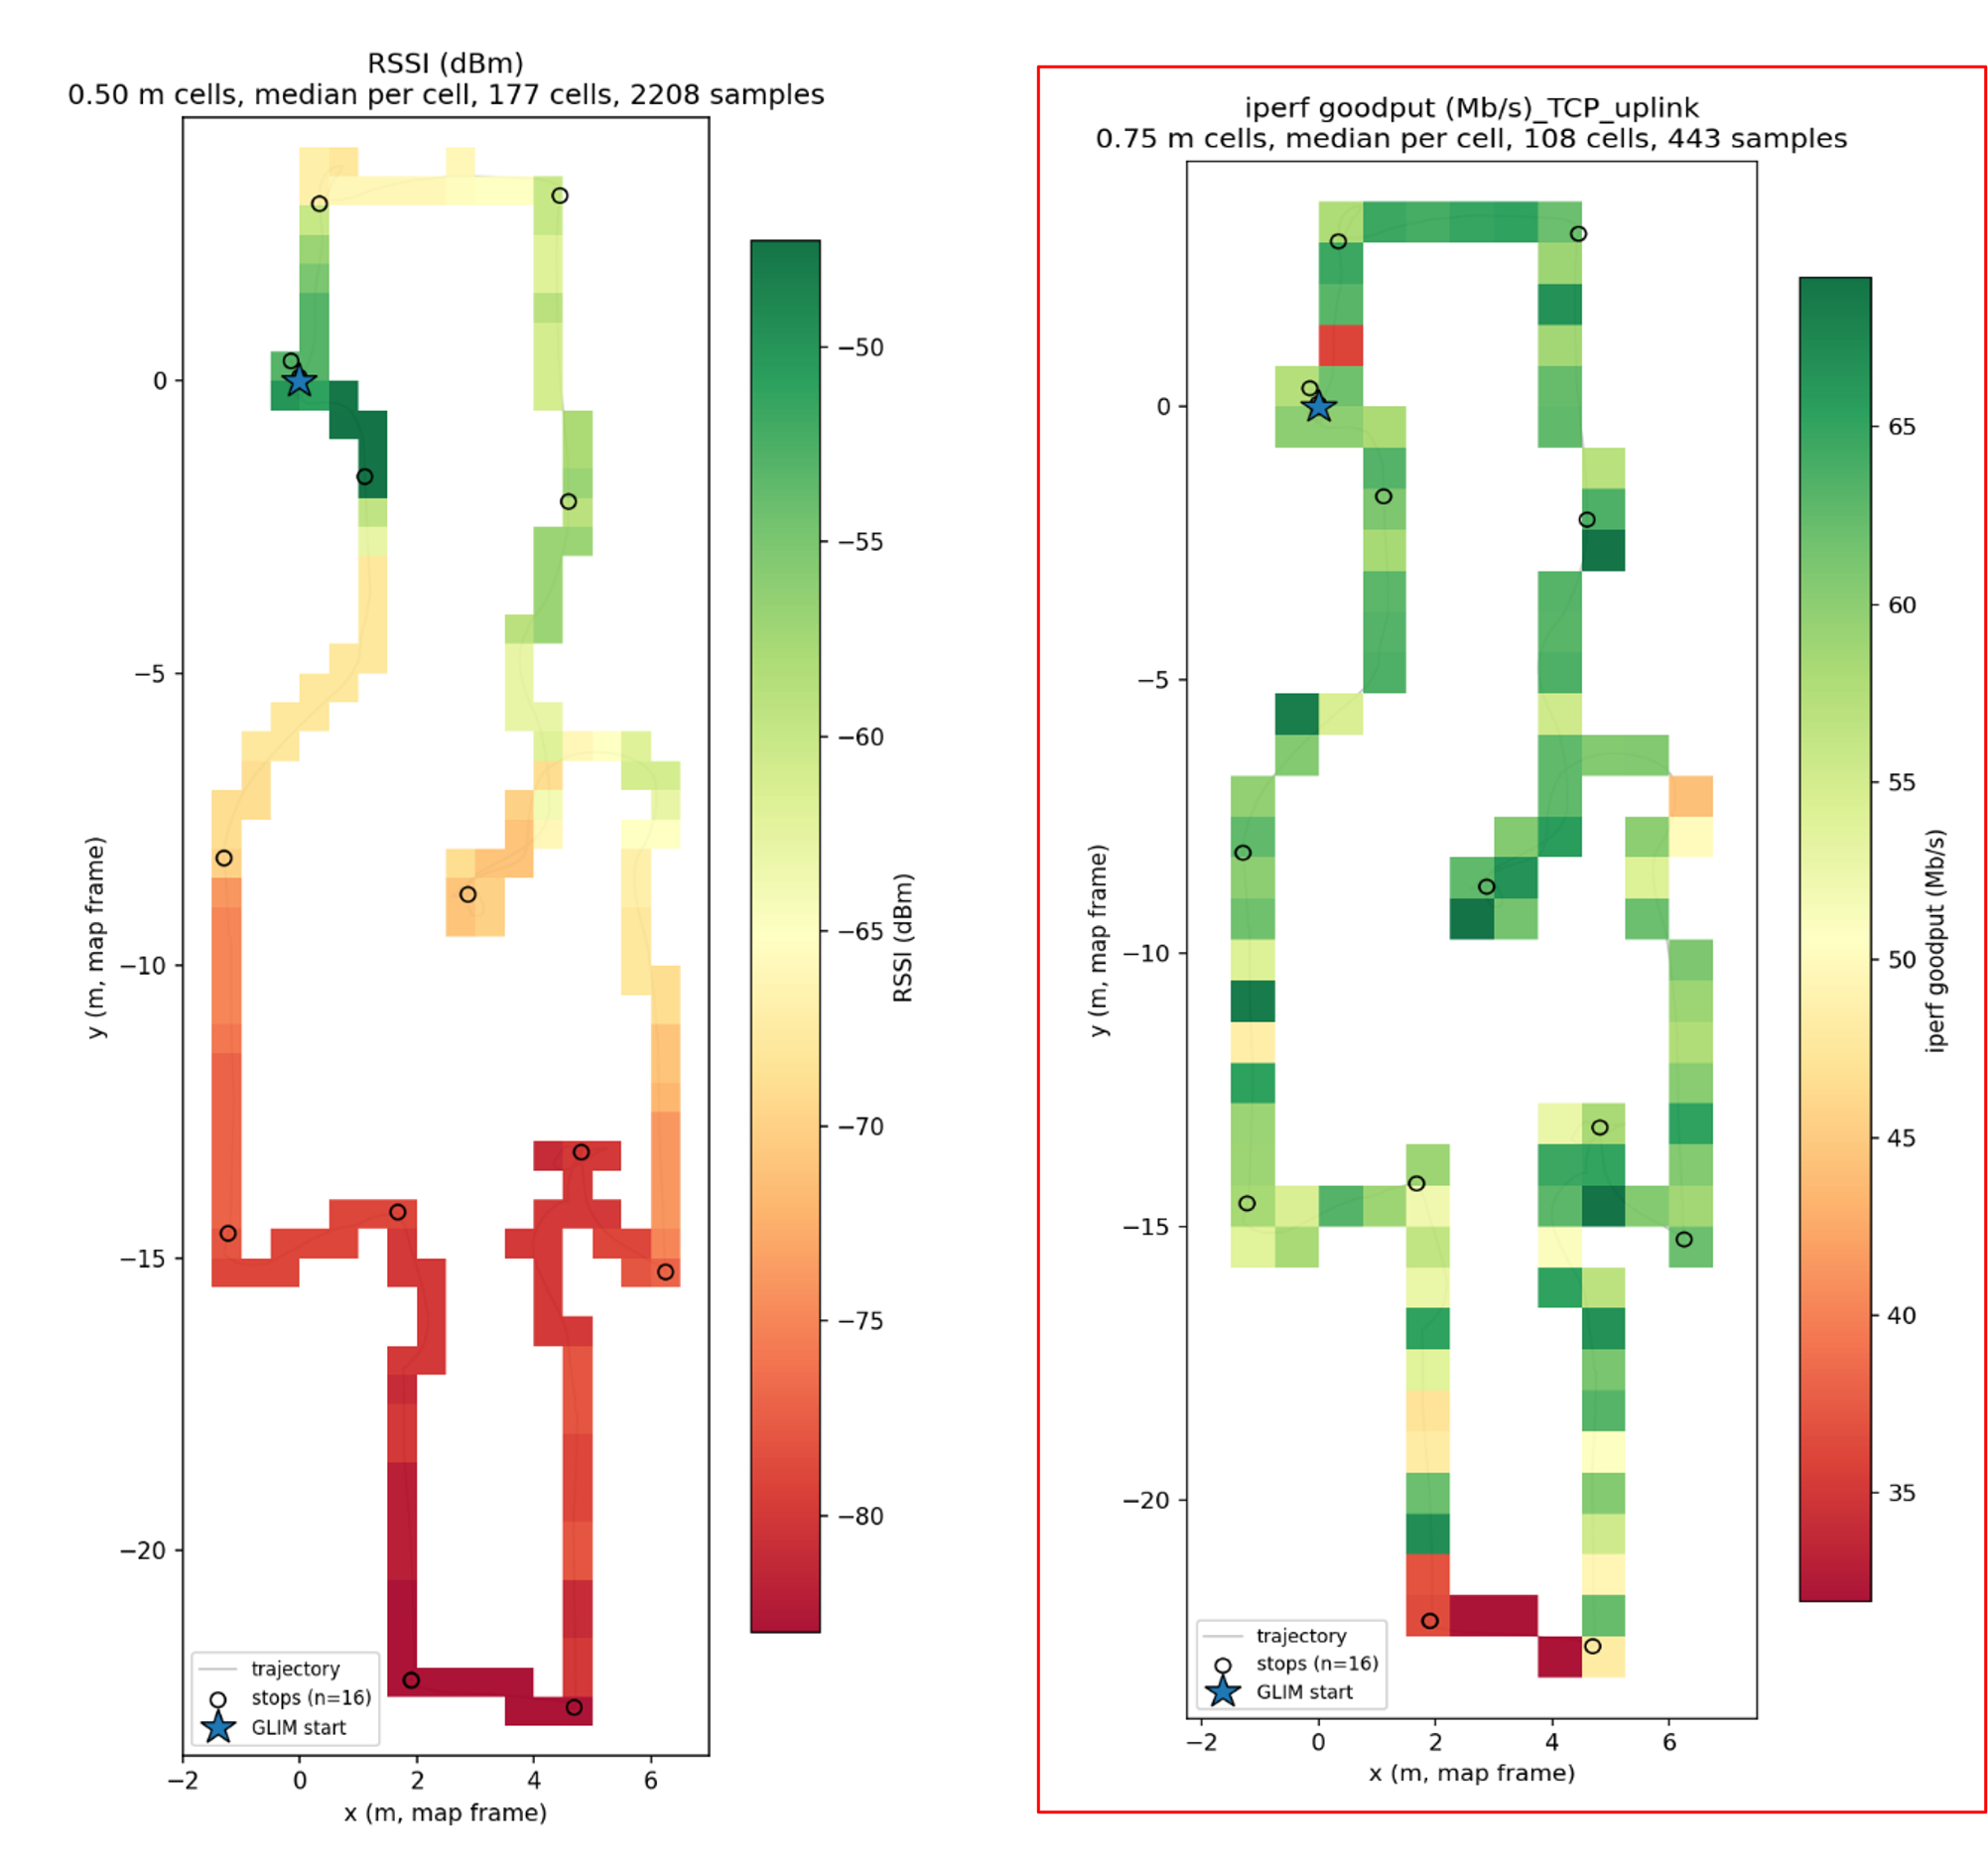
\includegraphics[width=\columnwidth]{figs/fig09_link_trace.png}
\caption{Measured link over one survey sequence at site 1, in the
reference map frame. Left: RSSI, median per \SI{0.5}{\metre} cell
(177 cells, 2208 samples). Right: TCP uplink goodput from
\texttt{iperf3}, median per \SI{0.75}{\metre} cell (108 cells, 443
samples). Circles mark the 16 survey stops, the star the start of the
mapping trajectory.}
\label{fig:linktrace}
\end{figure}


%=======================================================================
\section{Post-Processing Pipeline}
\label{sec:postproc}
Recording and release are separate stages. During a run, each unit
writes only what its sensors and interfaces produce. The per-unit
recordings are converted into a merged, time-aligned bag and derived
products by a fixed pipeline (Fig.~\ref{fig:dataflow}), run once per
sequence and released so that every step can be repeated.

\begin{figure*}[t]
\centering
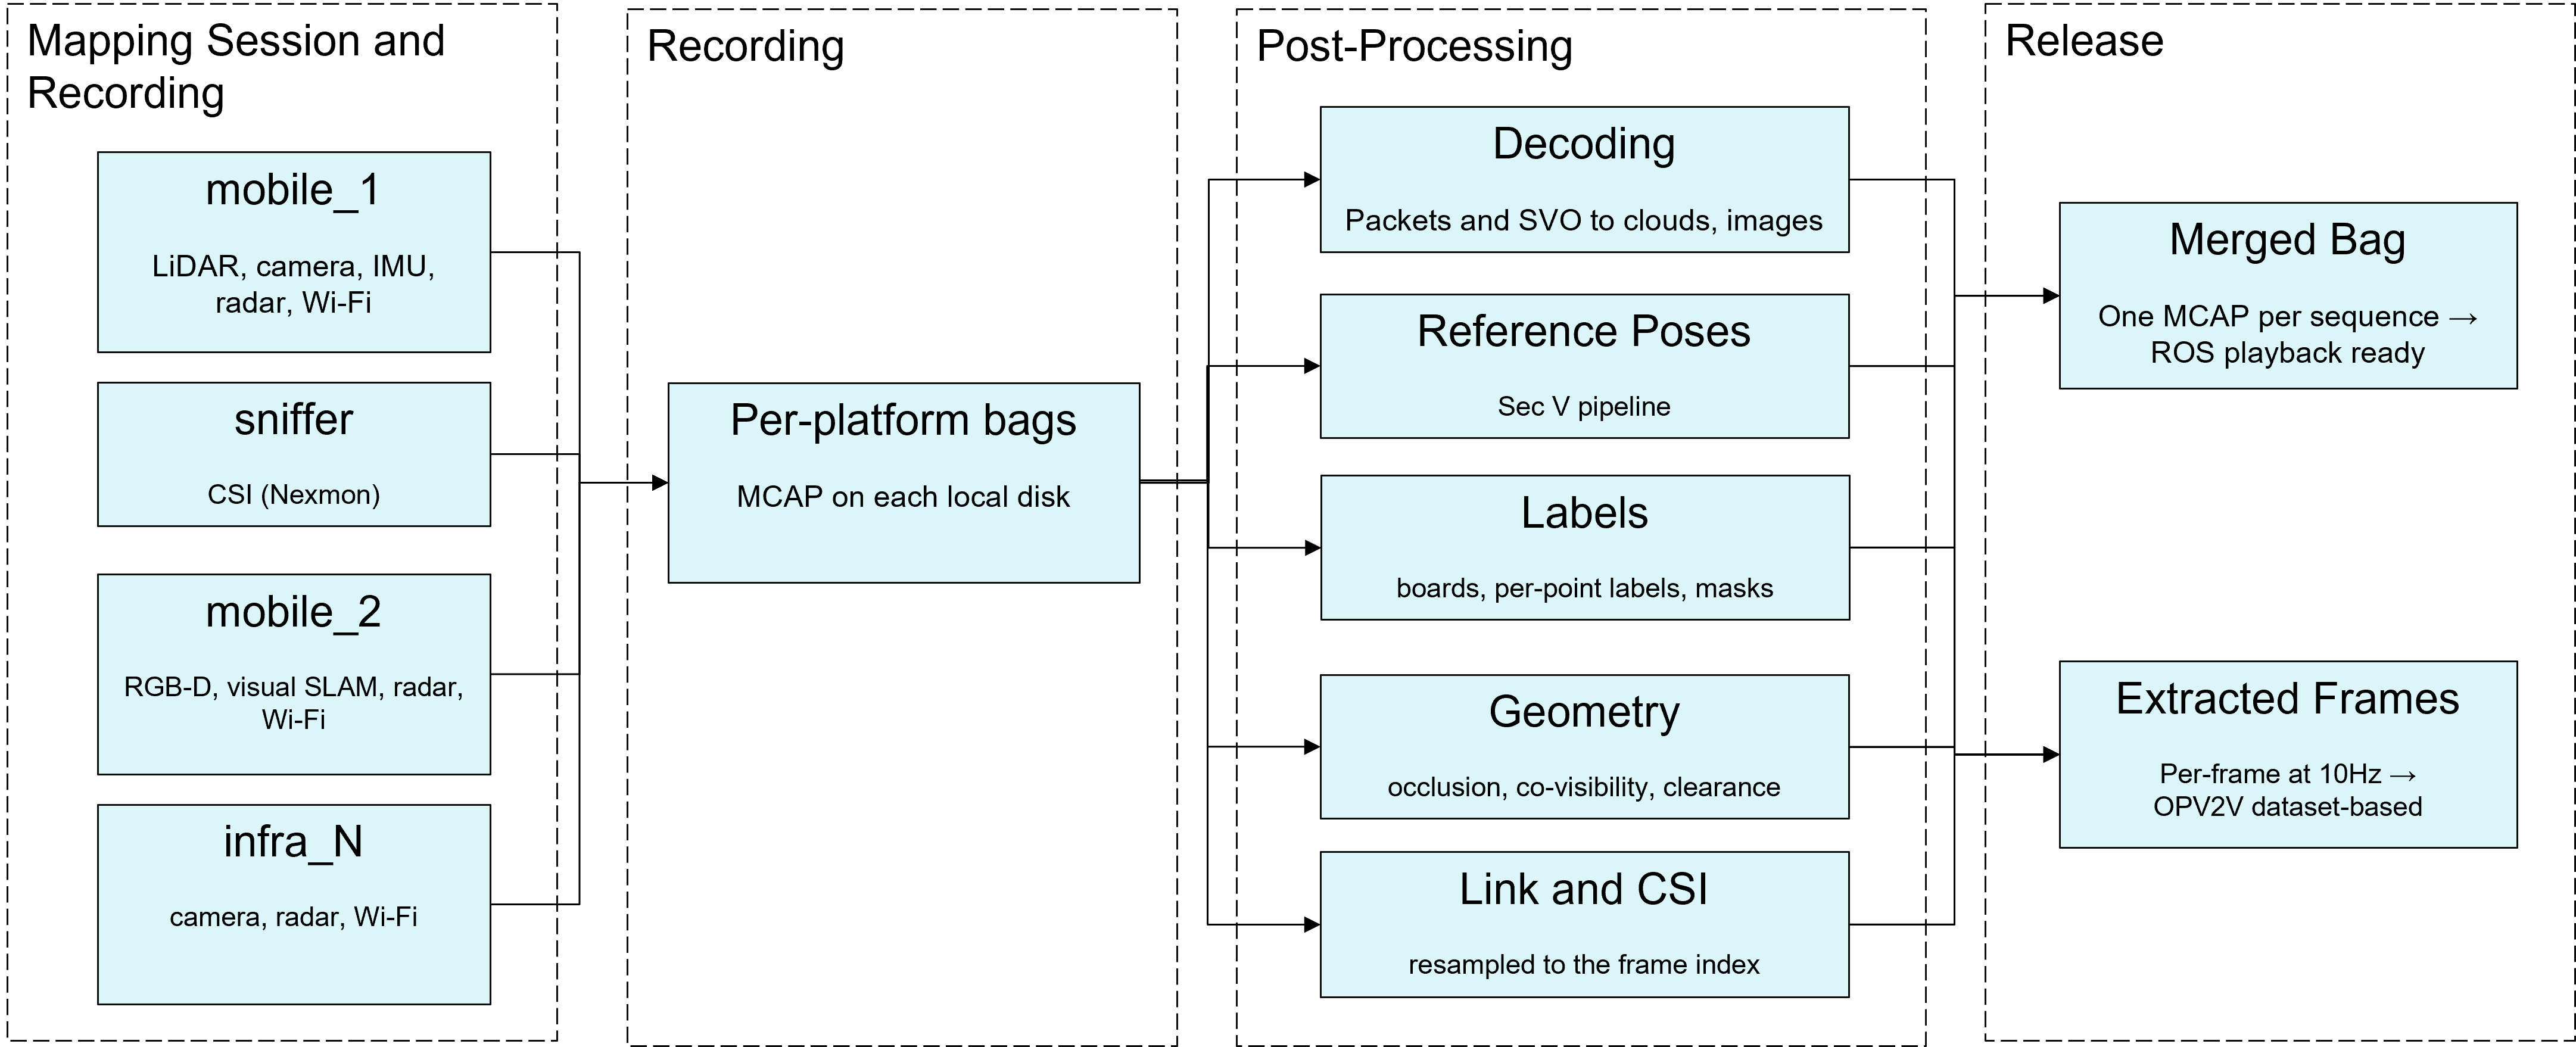
\includegraphics[width=\textwidth]{figs/fig03_dataflow.png}
\caption{Data flow from sensors to release files.}
\label{fig:dataflow}
\end{figure*}

\emph{Decoding.} The Ouster packets are decoded into \SI{10}{\hertz}
point clouds with the vendor driver and the sensor's metadata
message, using the same driver version as the reference pipeline. The
ZED~2i recordings, stored as \texttt{.svo} files, are decoded with the
ZED SDK into left and right images, depth, and IMU samples at their
native rates. The RealSense streams and the infrastructure cameras are
recorded as images and require no decoding. Every decoded message
keeps the stamp of the packet or frame it was decoded from.

\emph{Reference poses.} Each agent's pose in the site frame,
\texttt{global\_pose}, is computed offline by the reference pipeline
of Sec.~\ref{sec:groundtruth}: scan-to-map registration against the
frozen map for the LiDAR agents, depth-to-map registration with board
constraints for \texttt{mobile\_2}, and the fiducial chain of
Sec.~\ref{sec:fiducials} for the infrastructure. Poses are written at
the LiDAR or depth frame rate and can be interpolated to any other
sensor's stamps.

\emph{Link and channel.} The passive and active link metrics are
resampled to a common frame index, and the CSI frames captured by
\texttt{sniffer} are parsed from the Nexmon format into NumPy/HDF5
arrays and time-joined to the reference poses.

\emph{Merge.} The per-unit recordings, the decoded streams, the
reference poses and TF, and the parsed link state are written into a
single MCAP per sequence, ordered on the common timebase. Every
message carries its stamp converted to \texttt{mobile\_1}'s clock
using the offset logged by that unit at that moment
(\texttt{ntp/status}, \SI{10}{\hertz}), and the unit's original stamp
is preserved in the MCAP publish time, so users can recover the raw
per-unit timeline and can discard frames recorded while a unit's clock
offset exceeded a chosen threshold.

The annotation, collaboration-geometry, and per-frame extraction
stages that build on these products are part of the dataset release
and are described in \cite{scoop_dataset}.

%=======================================================================
\section{Evaluation}
\label{sec:evaluation}
We evaluate the testbed on the quantities a user of its data depends
on: the accuracy of the reference, the residuals of the calibration,
the stability of the clocks, and the character of the measured link.
All numbers come from recordings at three indoor sites on the Guangfu
Campus of National Yang Ming Chiao Tung University, which differ in
layout, corridor width, wall material, and access-point placement.

\subsection{Reference Accuracy}
\label{sec:eval_gt}
Table~\ref{tab:gt} and Fig.~\ref{fig:gt_errors} summarize the checks
of Sec.~\ref{sec:gt_val}.

\paragraph{Second mapping pass.} After refinement, floor surfaces are
within \SI{1}{\centi\metre} of the sensor noise floor, while walls,
observed at longer range and shallower incidence, remain above it.
The larger wall thickness of Sequence B comes from extended
single-visit corridor sections, where no revisit constrains the
lateral placement; floors, observed at short range throughout, are
unaffected. The second recording, captured four weeks later and
processed independently, reproduces the surface placement to
\SI{1.06}{\centi\metre} on walls, with the relative scale agreeing to
$2\times10^{-5}$.

\paragraph{Control distances.} \todo{Already measured some distances:
$N$ distances of \SIrange{5}{40}{\metre} per site. Report per site:
mean and max map-minus-rangefinder error.}

\paragraph{Held-out boards.} \todo{Report the median and
95th-percentile board residual, in translation and rotation, per
agent.}

\paragraph{Pose consistency.} \todo{Report repeat-visit and
cross-robot surface agreement for the LiDAR pair and for LiDAR against
RGB-D.}

No single number in Table~\ref{tab:gt} applies to every use of the
reference, and each number bounds one error only. A smooth
deformation displaces surfaces without thickening them, since the
scans remain locally consistent, so the residual thickness is per-scan
placement scatter, which averages out in the map. The cross-session
comparison bounds the disagreement between the surface placement of
two runs, here about one centimetre, and the control distances bound
the disagreement both runs have in common. Annotations placed against
the fused map therefore inherit centimetre-level geometry, while
per-scan placement scatter and pose-level fusion are governed by the
repeat-visit, cross-robot, and board figures. We release the
reference as a validated pseudo-ground truth on these terms: it is
established from onboard sensing alone, and the independent
measurements are used only to check the result, never to produce it.

\begin{table}[!t]
\centering
\caption{Pseudo Ground Truth Map Quality}
\label{tab:gt}
\begin{tabular}{llc}
\toprule
& Quantity & Value \\
\midrule
\multicolumn{3}{l}{\emph{Surface geometry}} \\
\quad Thickness, seq.\ A & walls / floors & 7.9 / 2.1 cm \\
\quad Thickness, seq.\ B & walls / floors & 9.7 / 2.4 cm \\
\quad Sensor noise floor & walls / floors & 2.9 / 1.25 cm \\
\quad Cross-session      & surface placement, walls & 1.06 cm \\
\quad Cross-session      & relative scale & 0.99998 \\
\quad Control distances  & rangefinder, median & -- \\
\midrule
\multicolumn{3}{l}{\emph{Pose consistency}} \\
\quad Refinement         & final pose correction & 0.15 cm, 0.017$^\circ$ \\
\quad Repeat-visit       & same robot & -- \\
\quad Cross-robot        & LiDAR vs.\ LiDAR & -- \\
\quad Cross-robot        & LiDAR vs.\ RGB-D & -- \\
\bottomrule
\end{tabular}
\end{table}


\begin{figure}[t]
\centering
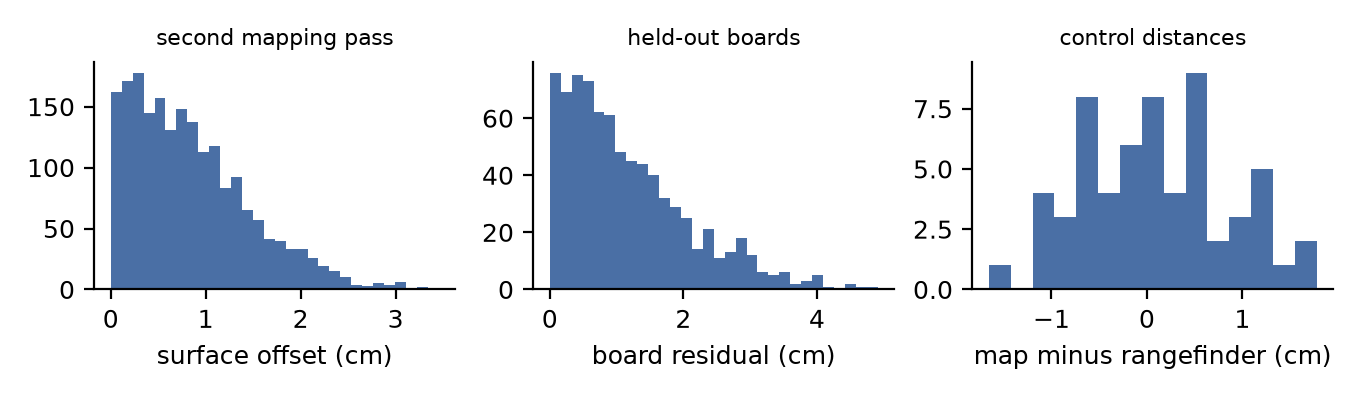
\includegraphics[width=\columnwidth]{figs/fig07_gt_errors.png}
\caption{Ground-truth error distributions from the three independent
checks. \todo{Dummy data.}}
\label{fig:gt_errors}
\end{figure}


\subsection{Calibration and Timing}
Table~\ref{tab:calib} reports the held-out residuals per transform
and the clock statistics. \todo{Discuss: which extrinsic is weakest
and why (radar, expected); whether the board-chain residual on
mobile\_1 is consistent with the LiDAR--camera residual alone, which
would show the hand-eye transform adds little error; the measured
sniffer bias against the \SI{7.8}{\milli\second} worst case.}

\subsection{Link Characterization}
\label{sec:eval_link}
Fig.~\ref{fig:linktrace} shows RSSI and uplink goodput over one survey
sequence, binned in the reference map frame. \todo{Report per site:
RSSI range, goodput range in survey and cooperation modes, RTT idle
and loaded, fraction of samples with \texttt{associated=false}, and
achieved CSI rates per transmitter. Show the contention effect:
goodput per agent in cooperation mode against survey mode on the same
route.}

\subsection{Geometric Link State Against Measured RSSI}
\label{sec:eval_clear}
The dataset built on this testbed \cite{scoop_dataset} labels each
link per frame with its first-Fresnel-zone clearance computed from the
reference map, independently of the measured signal. The testbed makes
that independence testable: because the map, the poses, and the RSSI
are all recorded, the geometric label can be checked against the
signal it is meant to predict. \todo{Report RSSI distribution for
frames with clearance above and below 0.6, per site; this is the
check that a map-derived link label carries information about the
measured link.}

\subsection{End-to-End Demonstration}
\todo{One sequence shown from raw bags to merged MCAP: timeline of all
units, reference trajectories on the map, link trace, and CSI
amplitude over time, to show that the products of
Sec.~\ref{sec:postproc} line up on one timebase. Optionally a
single-agent SLAM run (GLIM on mobile\_1, on-board VSLAM on mobile\_2)
evaluated against the reference to demonstrate use as an evaluation
target.}

%=======================================================================
\section{Lessons Learned and Limitations}
\label{sec:lessons}

\paragraph{The CSI receiver dictates the network.} Commodity CSI
extraction imposed a single spatial stream, 802.11ac rather than ax,
and \SI{80}{\mega\hertz} bandwidth on every transmitter. These are
constraints of the measurement, not of the robots, and they must be
stated with any throughput number recorded on the platform.

\paragraph{Aggregation caps the CSI rate.} One channel estimate per
aggregated transmission limits CSI to roughly \SIrange{100}{140}{\hertz}
under load, sufficient only below about \SI{1.2}{\metre\per\second} of
relative motion. Raising the rate by disabling aggregation would
distort the throughput being measured; the two cannot be optimized
together on one link.

\paragraph{Keep the sniffer off a second wireless hop.} Synchronizing
the CSI host over a \SI{2.4}{\giga\hertz} management link introduced
the only clock bias the protocol cannot observe. The probe-packet
measurement bounds it, but a wired connection to \texttt{mobile\_1}
removes it. \todo{Confirm once the Ethernet change is made.}

\paragraph{Plane targets, not nearest neighbours.} On a map smeared by
drift, nearest-neighbour ICP hides a \SI{3}{\centi\metre} scan offset
behind a \SI{0.5}{\centi\metre} residual. Registration against local
plane fits made the error visible and was necessary to reach the
reported surface thickness.

\paragraph{Post boards from the map, not from a survey.} Estimating
board poses from the mapping session itself removed the survey
instrument and gave the RGB-D agent and the infrastructure a frame
consistent with the LiDAR map by construction. The cost is that board
accuracy is bounded by map accuracy, which is why the control
distances are needed.

\paragraph{Limitations.} The radio layer covers one band, one
protocol, and one access point per site, with CSI from a single
receiver. The two mapping passes share a sensor and a pipeline, so
absolute accuracy rests on the control distances. Each extrinsic is
validated on held-out observations but the rig, once fixed, is not
re-verified per session. \todo{Add scale: three sites, number of
sessions and hours recorded, once final.}

%=======================================================================
\section{Conclusion}
\label{sec:conclusion}
We presented a heterogeneous indoor multi-robot testbed in which the
wireless link between every pair of agents is measured on the sensing
timeline and every agent, with or without a LiDAR, is placed in one
building-scale metric frame built from the testbed's own sensors and
validated against independent measurements. The calibration and timing
budget shows that synchronization is not the limiting error, and the
reference reaches centimetre-level surface agreement across
independent passes. The platform is the acquisition system of the
SCooP dataset \cite{scoop_dataset}; its post-processing pipeline is
released so that the products described here can be regenerated.
Future work includes a wired CSI host, multi-antenna CSI extraction,
and additional access points per site.

\section*{Acknowledgment}
\todo{Add acknowledgments in this section.}

\bibliographystyle{IEEEtran}
\bibliography{references}

\appendices
\section{Sensor Intrinsics}
\label{app:intrinsics}
\todo{Per-sensor intrinsic parameters and the plots behind
Table~\ref{tab:calib}: camera reprojection residual by image region,
LiDAR range bias by range, radar reflector offset by range.}

%\begin{figure}[t]
\centering
\fbox{\parbox[c][4cm][c]{0.95\columnwidth}{\centering
\todo{Fig.~19: per-sensor intrinsic calibration plots.}}}
\caption{Intrinsic calibration residuals per sensor.}
\label{fig:app_intrinsics}
\end{figure}


\section{Bill of Materials}
\label{app:bom}
\todo{Per-agent component list with approximate cost, to support the
claim that the reference is reachable without a survey scanner.}

\end{document}
